
We can now add Jupiter to the system, so that we have a three-body problem. We
want to see how much Jupiter alters Earth's motion. We choose the same
parameters as we did for the stable orbit in the Sun-Earth system, so $\D t =
0.01$ and we simulate over a period of $T = 100$ years. Again we assume circular
orbits, and choose initial velocities from this. The Sun-Earth-Jupiter
system can be seen in figure \refig{sunEarthJupiter}.
%
\begin{figure}[htpb]
	\centering
	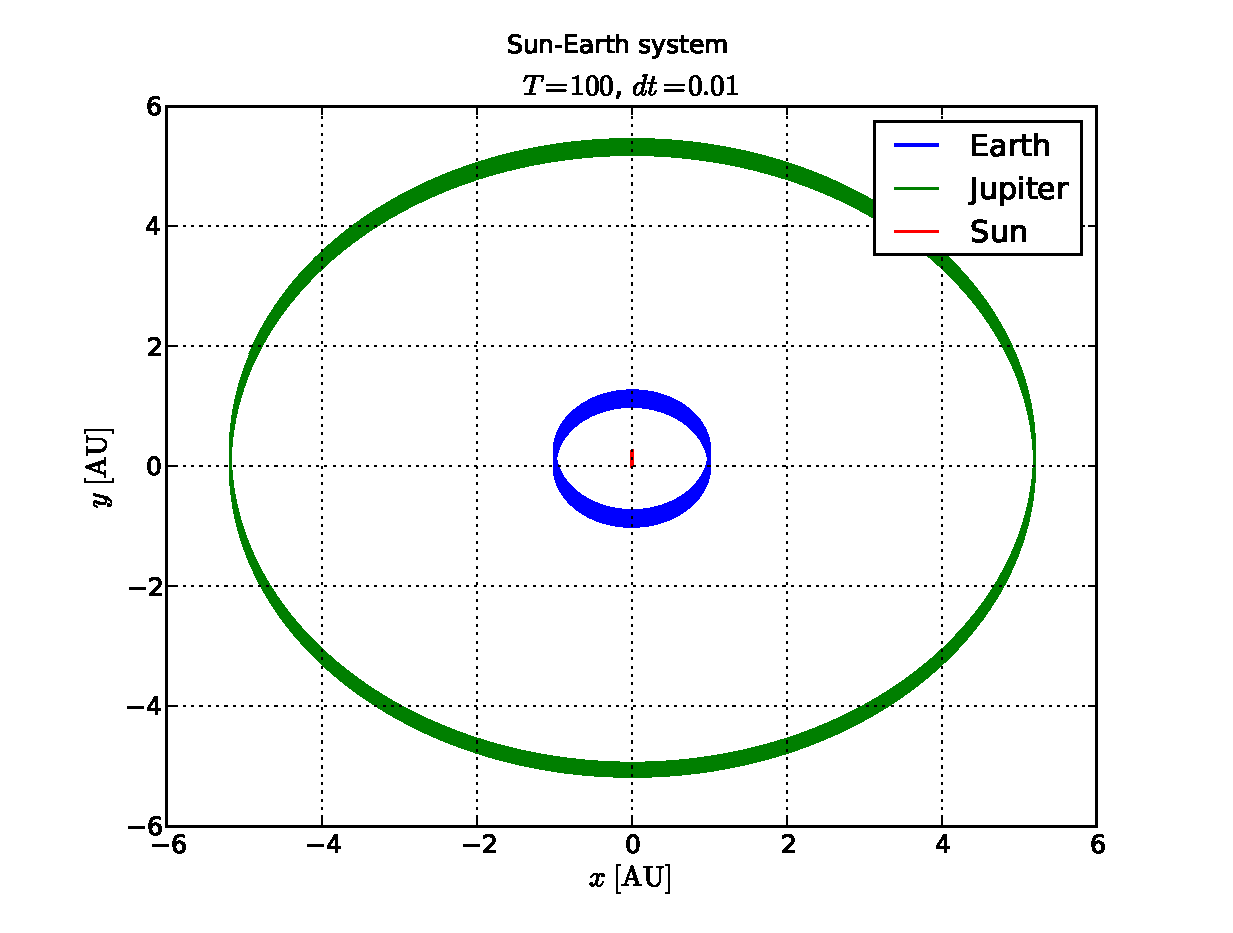
\includegraphics[width=0.8\textwidth]{figures/sun_earth_jupiter_dt1e-2}
	\caption{The Sun-Earth-Jupiter system simulated over $T = 100$ years, with
	time step $\D t = 0.01$.}
	\label{fig:sunEarthJupiter}
\end{figure}
%
We can clearly see that Jupiter alters Earth's motion, comparing the two
figures \refig{sunEarth-dt0.01} and \refig{sunEarthJupiter}. The orbit of Earth
is much less restricted, resulting in some variation, depending on where Jupiter
is at any given time. We increase the time step to $\D t = 0.1$ as
we did earlier, and see that it is high enough to cause RK4 to fail for the
Earth, while Jupiter's orbit remains unaltered. See figure
\refig{sunEarthJupiter-dt1e-2}
%
\begin{figure}[htpb]
	\centering
	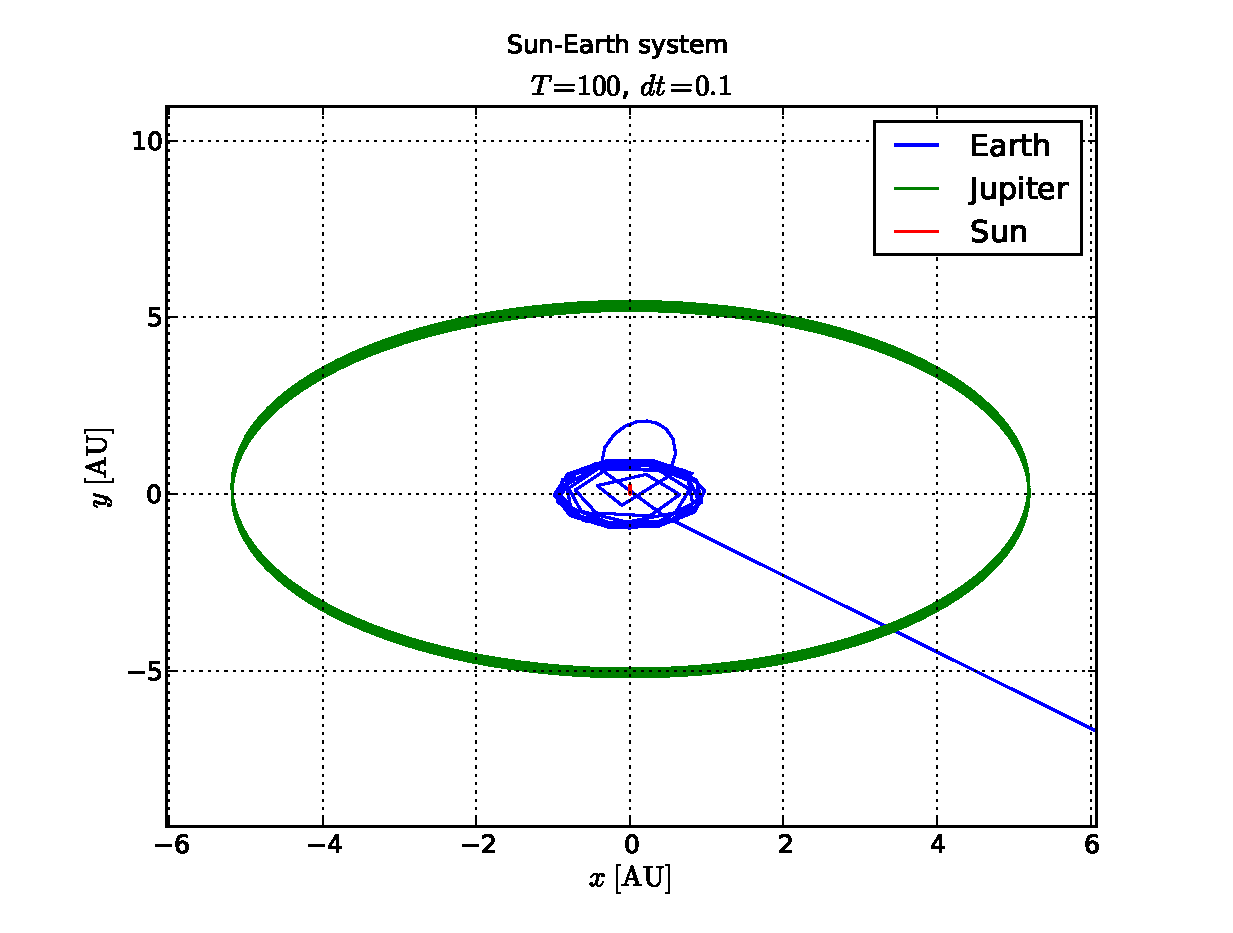
\includegraphics[width=0.8\textwidth]{figures/sun_earth_jupiter_dt1e-1}
	\caption{Sun-Earth-Jupiter system with $\D t = 0.1$, which causes RK4 to fail
	in calculating Earth's orbit. Jupiter's orbit remains unaltered.}
	\label{fig:sunEarthJupiter-dt1e-2}
\end{figure}
%
We increase the mass of Jupiter by factors of $10$ and $1000$, and see how this
affects Earth's motion. The results are shown in figures \refig{jupiter10} and
\refig{jupiter1000}.
%
\begin{figure}[htpb]
	\centering
	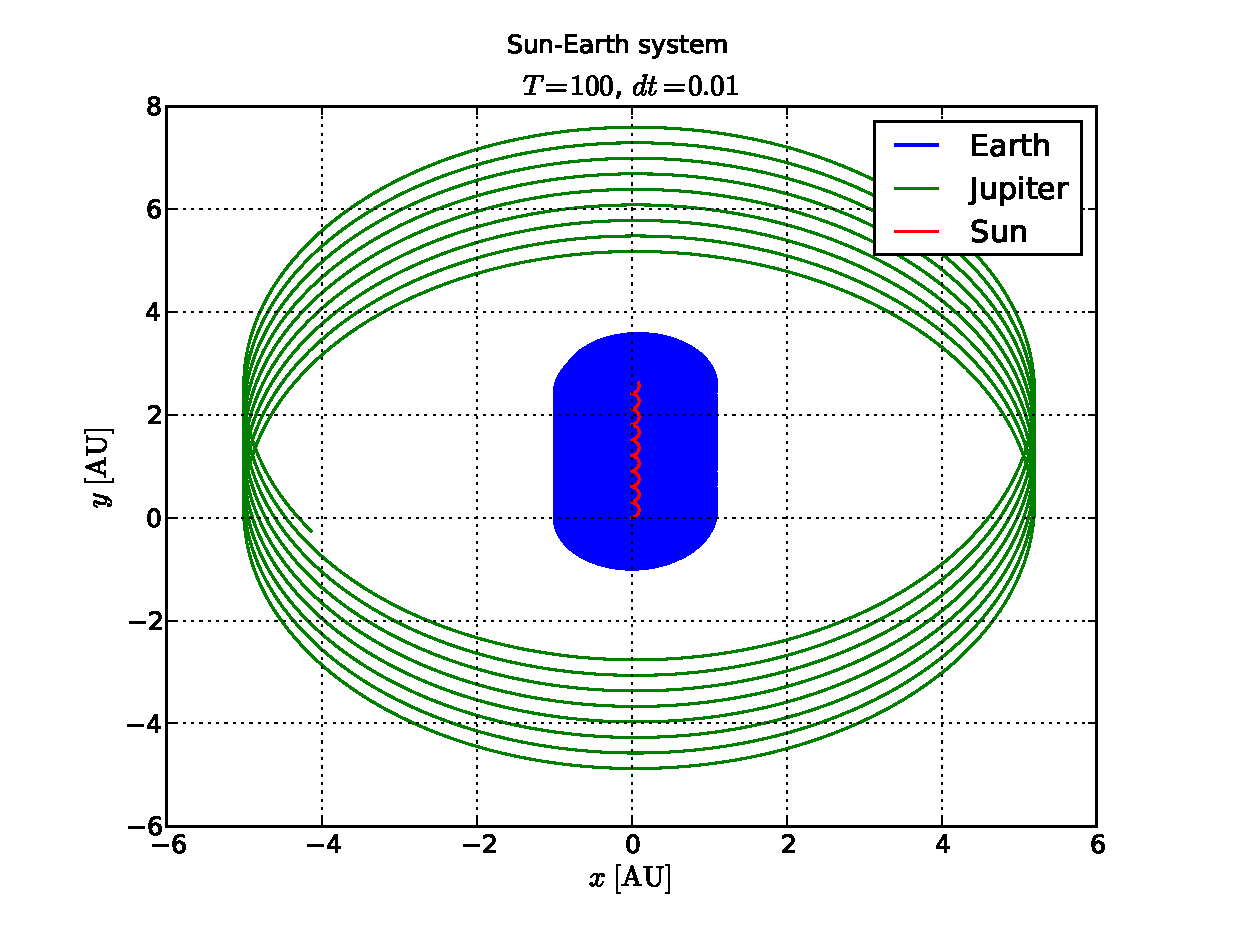
\includegraphics[width=0.8\textwidth]{figures/sun_earth_jupiter_incmass10}
	\caption{Sun-Earth-Jupiter system with an increase in Jupiter's mass by a
	factor of 10.}
	\label{fig:jupiter10}
\end{figure}
%
\begin{figure}[htpb]
	\centering
	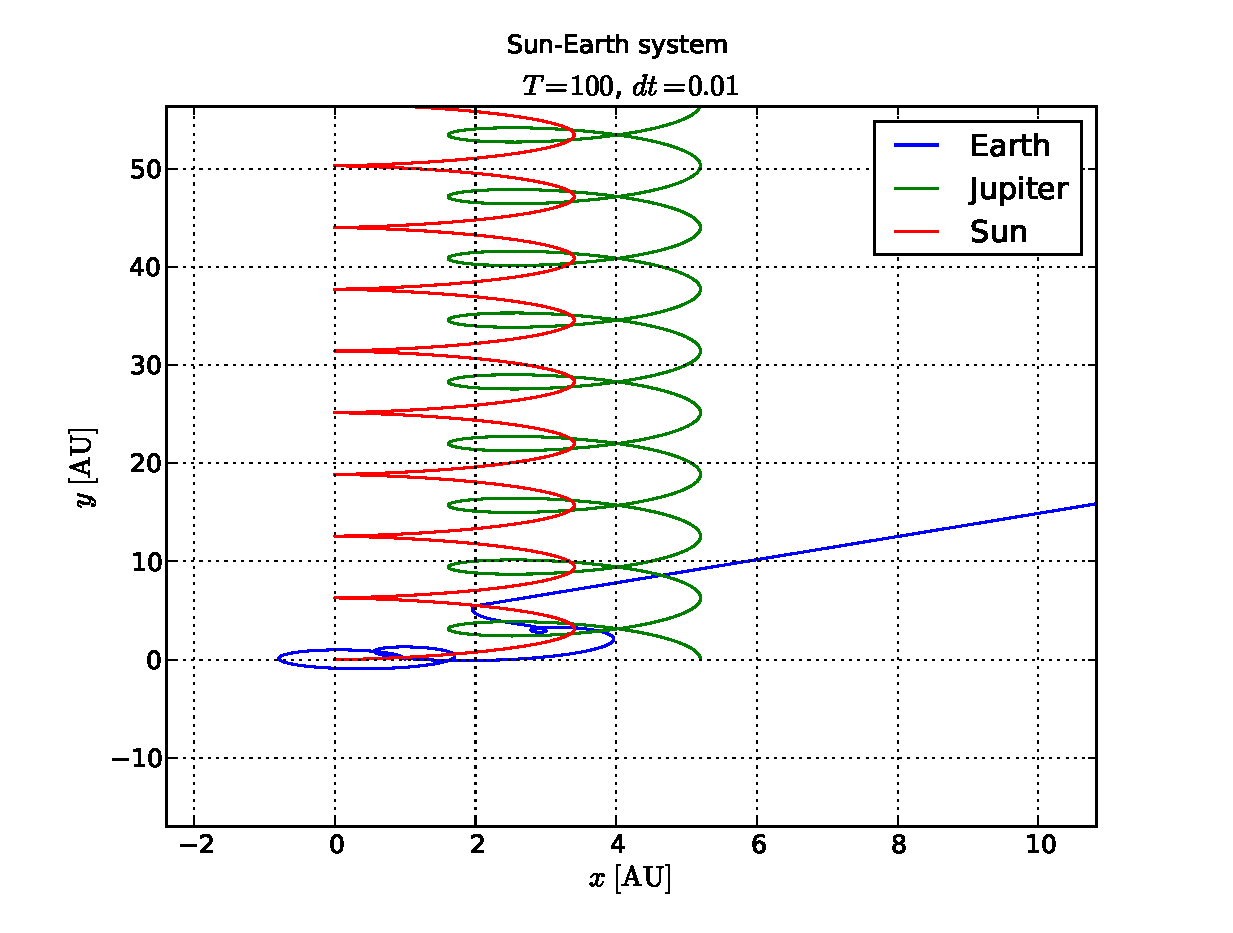
\includegraphics[width=0.8\textwidth]{figures/sun_earth_jupiter_incmass1000}
	\caption{Sun-Earth-Jupiter system with an increase in Jupiter's mass by a
	factor of 1000.}
	\label{fig:jupiter1000}
\end{figure}
%
From figure \refig{jupiter10} we see that all three objects move upwards. This
is most likely due to the fact that we haven't set the Sun's acceleration to
always be zero, such that it gains momentum now that Jupiter has a much larger
mass, and therefore takes both Earth and Jupiter with it. More discussion on
this will follow later.

We also see from figure \refig{jupiter1000} that the almost same thing happens.
The Sun's motion brings Jupiter with it, while Earth gains a very large velocity
at one point, resulting in it leaving the system.

Although increasing Jupiter's mass by a significant amount does lead to strange
orbits, the stability of the program seems to remain unchanged to some degree.
Earth still shoots out of the system at the same time steps as in the Sun-Earth
system.

